\documentclass[journal]{IEEEtran}
\usepackage[a5paper, margin=10mm, onecolumn]{geometry}
%\usepackage{lmodern} % Ensure lmodern is loaded for pdflatex
\usepackage{tfrupee} % Include tfrupee package

\setlength{\headheight}{1cm} % Set the height of the header box
\setlength{\headsep}{0mm}     % Set the distance between the header box and the top of the text

\usepackage{gvv-book}
\usepackage{gvv}
\usepackage{cite}
\usepackage{amsmath,amssymb,amsfonts,amsthm}
\usepackage{algorithmic}
\usepackage{graphicx}
\usepackage{textcomp}
\usepackage{xcolor}
\usepackage{txfonts}
\usepackage{listings}
\usepackage{enumitem}
\usepackage{mathtools}
\usepackage{gensymb}
\usepackage{comment}
\usepackage[breaklinks=true]{hyperref}
\usepackage{tkz-euclide} 
\usepackage{listings}
% \usepackage{gvv}                                        
\def\inputGnumericTable{}                                 
\usepackage[latin1]{inputenc}                                
\usepackage{color}                                            
\usepackage{array}                                            
\usepackage{longtable}                                       
\usepackage{calc}                                             
\usepackage{multirow}                                         
\usepackage{hhline}                                           
\usepackage{ifthen}                                           
\usepackage{lscape}
\begin{document}

\bibliographystyle{IEEEtran}
\vspace{3cm}

\title{11.16.3.2}
\author{EE24BTECH11001 - Aditya Tripathy}
 \maketitle
% \newpage
% \bigskip
{\let\newpage\relax\maketitle}

\renewcommand{\thefigure}{\theenumi}
\renewcommand{\thetable}{\theenumi}
\setlength{\intextsep}{10pt} % Space between text and floats


\numberwithin{equation}{enumi}
\numberwithin{figure}{enumi}
\renewcommand{\thetable}{\theenumi}


\textbf{Question}:\\
A coin is tossed twice, what is the probability that atleast one tail occurs?
\\
\textbf{Solution :}\\
Let Y be the random variable representing the number of tails. Y can be represented as the sum of two bernoulli random variables, $X_1, X_2$,
\begin{align}
  Y = X_1 + X_2
\end{align}
The Bernoulli R.V is defined as,
\begin{align}
	X_i = \begin{cases}
		0 & \text{Outcome is Heads}\\	
		1 & \text{Outcome is Tails}	
	\end{cases}
\end{align}
The PMF of Bernoulli R.V is given by,
\begin{align}
  p_X\brak{n} = \begin{cases}
    p & n = 0\\
    1-p & n = 1
  \end{cases}
\end{align}
Using properties of Z transform of PMF on eq. \brak{0.1},
\begin{align}
  M_Y\brak{z} &= M_{X_1}\brak{z}M_{X_2}\brak{z}\\
  M_{X_1}\brak{z} &= \sum_{k = -\infty}^{\infty} p_{X_1}\brak{k}z^{-k} = p + \brak{1-p}z^{-1}\\
  M_{X_2}\brak{z} &= \sum_{k = -\infty}^{\infty} p_{X_2}\brak{k}z^{-k} = p + \brak{1-p}z^{-1}\\
  M_Y\brak{z} &= \brak{p + \brak{1-p}z^{-1}}^2\\
              &= \sum_{k = -\infty}^{\infty} \comb{2}{k}p^{2-k}\brak{1-p}^{k}z^{-k}\\
  p_Y\brak{n} &= \comb{2}{n} p^{2-n}\brak{1-p}^n
\end{align}
Substituting $p = \frac{1}{2}$,
\begin{align}
  p_Y\brak{n} &= \comb{2}{n}\brak{\frac{1}{2}}^2
\end{align}

Using eq. (0.9) the CDF (Cumulative Distribution Function) is given by:
\begin{align}
  F_{X}\brak{n} = \sum_{k = -\infty}^n\comb{2}{k}\brak{\frac{1}{2}}^2 = \begin{cases}
    0 & x < 0\\
    \comb{2}{0}\brak{\frac{1}{2}}^2 = \frac{1}{4} & 0 \le x < 1\\
    \comb{2}{1}\brak{\frac{1}{2}}^2 + \comb{2}{0}\brak{\frac{1}{2}}^2 = \frac{3}{4}& 1 \le x < 2\\
    \comb{2}{2}\brak{\frac{1}{2}}^2 + \comb{2}{1}\brak{\frac{1}{2}}^2 + \comb{2}{0}\brak{\frac{1}{2}}^2 = 1 & x >=2\\
  \end{cases}
\end{align}
\begin{align}
  p\brak{X \ge 1} &= 1 - p\brak{X < 1}\\
  &= 1 - \frac{1}{4} = \frac{3}{4}
\end{align}
Simulation:
\newline
To run a simulation we need to generate random numbers with uniform probability, which is done
as shown below(Algorithm taken from OpenSSL's random\_uniform.c):
\begin{enumerate}
  \item \text{Generate 1byte(8 bits) of entropy using OpenSSL/rand.h.}
  \item Scale down this number in the range [0, 255] to [0, 1]by dividing by 255.
  \item Return 0 if the scaled down number is less than p and return 1 otherwise. 
\end{enumerate}
The following shows how the relative frequency reaches true probability with increasing number of trials of the event. The blue plot is the $n = 2$ case and red plot is the $n = 10$ case.
\begin{figure}[h!]
   \centering
   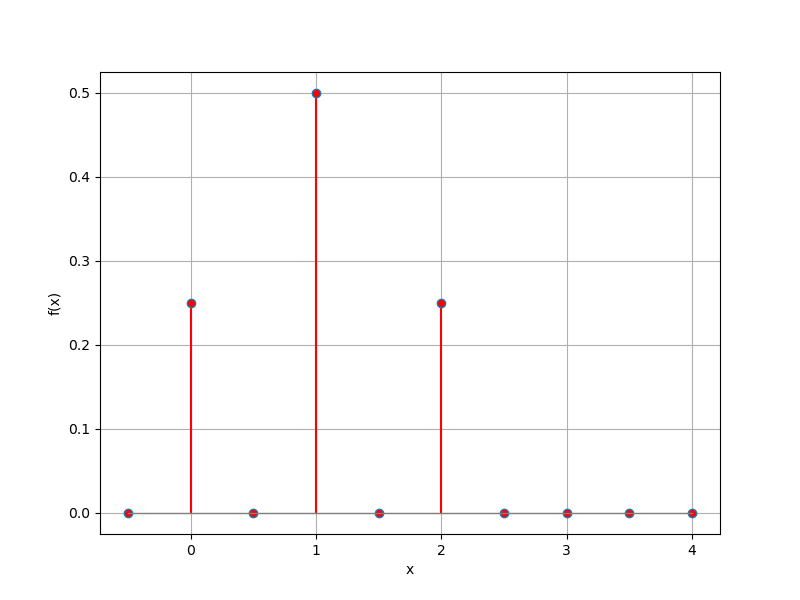
\includegraphics[width=0.7\columnwidth]{figs/fig1.png}
    \caption{Probability Mass Function}
\end{figure}
\begin{figure}[h!]
   \centering
   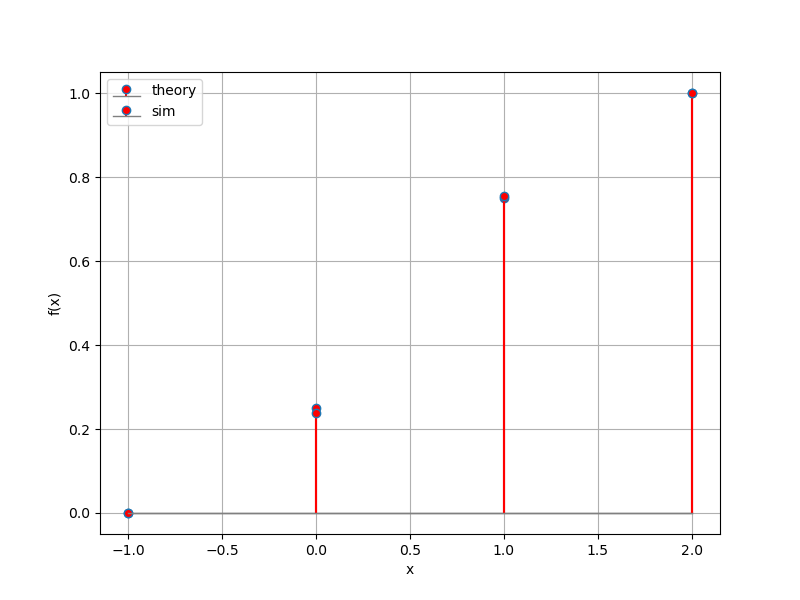
\includegraphics[width=0.7\columnwidth]{figs/fig2.png}
    \caption{Cumulative Distribution Function}
\end{figure}
\begin{figure}[h!]
   \centering
   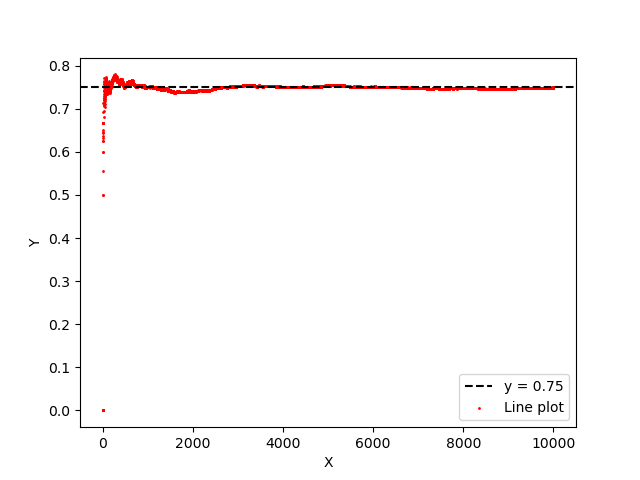
\includegraphics[width=0.7\columnwidth]{figs/fig.png}
    \caption{Relative Frequency tends to True Probability}
\end{figure}
\begin{figure}[h!]
   \centering
   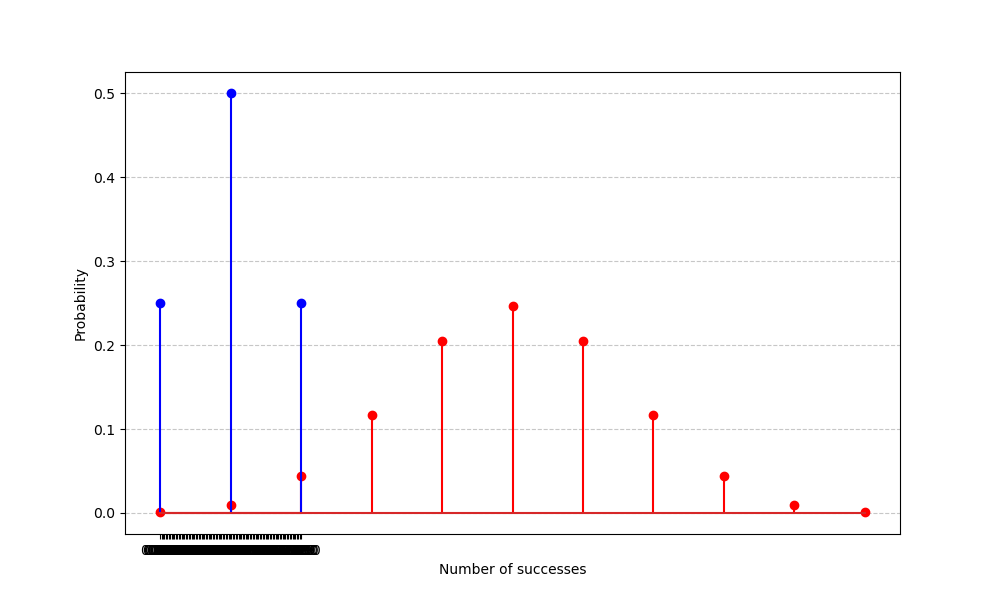
\includegraphics[width=0.7\columnwidth]{figs/binomial.png}
    \caption{Generating binomial distribution from bernoulli}
\end{figure}
\end{document}

